% Options for packages loaded elsewhere
\PassOptionsToPackage{unicode}{hyperref}
\PassOptionsToPackage{hyphens}{url}
\PassOptionsToPackage{dvipsnames,svgnames,x11names}{xcolor}
%
\documentclass[
  letterpaper,
  DIV=11,
  numbers=noendperiod]{scrreprt}

\usepackage{amsmath,amssymb}
\usepackage{iftex}
\ifPDFTeX
  \usepackage[T1]{fontenc}
  \usepackage[utf8]{inputenc}
  \usepackage{textcomp} % provide euro and other symbols
\else % if luatex or xetex
  \usepackage{unicode-math}
  \defaultfontfeatures{Scale=MatchLowercase}
  \defaultfontfeatures[\rmfamily]{Ligatures=TeX,Scale=1}
\fi
\usepackage{lmodern}
\ifPDFTeX\else  
    % xetex/luatex font selection
\fi
% Use upquote if available, for straight quotes in verbatim environments
\IfFileExists{upquote.sty}{\usepackage{upquote}}{}
\IfFileExists{microtype.sty}{% use microtype if available
  \usepackage[]{microtype}
  \UseMicrotypeSet[protrusion]{basicmath} % disable protrusion for tt fonts
}{}
\makeatletter
\@ifundefined{KOMAClassName}{% if non-KOMA class
  \IfFileExists{parskip.sty}{%
    \usepackage{parskip}
  }{% else
    \setlength{\parindent}{0pt}
    \setlength{\parskip}{6pt plus 2pt minus 1pt}}
}{% if KOMA class
  \KOMAoptions{parskip=half}}
\makeatother
\usepackage{xcolor}
\setlength{\emergencystretch}{3em} % prevent overfull lines
\setcounter{secnumdepth}{5}
% Make \paragraph and \subparagraph free-standing
\ifx\paragraph\undefined\else
  \let\oldparagraph\paragraph
  \renewcommand{\paragraph}[1]{\oldparagraph{#1}\mbox{}}
\fi
\ifx\subparagraph\undefined\else
  \let\oldsubparagraph\subparagraph
  \renewcommand{\subparagraph}[1]{\oldsubparagraph{#1}\mbox{}}
\fi

\usepackage{color}
\usepackage{fancyvrb}
\newcommand{\VerbBar}{|}
\newcommand{\VERB}{\Verb[commandchars=\\\{\}]}
\DefineVerbatimEnvironment{Highlighting}{Verbatim}{commandchars=\\\{\}}
% Add ',fontsize=\small' for more characters per line
\usepackage{framed}
\definecolor{shadecolor}{RGB}{241,243,245}
\newenvironment{Shaded}{\begin{snugshade}}{\end{snugshade}}
\newcommand{\AlertTok}[1]{\textcolor[rgb]{0.68,0.00,0.00}{#1}}
\newcommand{\AnnotationTok}[1]{\textcolor[rgb]{0.37,0.37,0.37}{#1}}
\newcommand{\AttributeTok}[1]{\textcolor[rgb]{0.40,0.45,0.13}{#1}}
\newcommand{\BaseNTok}[1]{\textcolor[rgb]{0.68,0.00,0.00}{#1}}
\newcommand{\BuiltInTok}[1]{\textcolor[rgb]{0.00,0.23,0.31}{#1}}
\newcommand{\CharTok}[1]{\textcolor[rgb]{0.13,0.47,0.30}{#1}}
\newcommand{\CommentTok}[1]{\textcolor[rgb]{0.37,0.37,0.37}{#1}}
\newcommand{\CommentVarTok}[1]{\textcolor[rgb]{0.37,0.37,0.37}{\textit{#1}}}
\newcommand{\ConstantTok}[1]{\textcolor[rgb]{0.56,0.35,0.01}{#1}}
\newcommand{\ControlFlowTok}[1]{\textcolor[rgb]{0.00,0.23,0.31}{#1}}
\newcommand{\DataTypeTok}[1]{\textcolor[rgb]{0.68,0.00,0.00}{#1}}
\newcommand{\DecValTok}[1]{\textcolor[rgb]{0.68,0.00,0.00}{#1}}
\newcommand{\DocumentationTok}[1]{\textcolor[rgb]{0.37,0.37,0.37}{\textit{#1}}}
\newcommand{\ErrorTok}[1]{\textcolor[rgb]{0.68,0.00,0.00}{#1}}
\newcommand{\ExtensionTok}[1]{\textcolor[rgb]{0.00,0.23,0.31}{#1}}
\newcommand{\FloatTok}[1]{\textcolor[rgb]{0.68,0.00,0.00}{#1}}
\newcommand{\FunctionTok}[1]{\textcolor[rgb]{0.28,0.35,0.67}{#1}}
\newcommand{\ImportTok}[1]{\textcolor[rgb]{0.00,0.46,0.62}{#1}}
\newcommand{\InformationTok}[1]{\textcolor[rgb]{0.37,0.37,0.37}{#1}}
\newcommand{\KeywordTok}[1]{\textcolor[rgb]{0.00,0.23,0.31}{#1}}
\newcommand{\NormalTok}[1]{\textcolor[rgb]{0.00,0.23,0.31}{#1}}
\newcommand{\OperatorTok}[1]{\textcolor[rgb]{0.37,0.37,0.37}{#1}}
\newcommand{\OtherTok}[1]{\textcolor[rgb]{0.00,0.23,0.31}{#1}}
\newcommand{\PreprocessorTok}[1]{\textcolor[rgb]{0.68,0.00,0.00}{#1}}
\newcommand{\RegionMarkerTok}[1]{\textcolor[rgb]{0.00,0.23,0.31}{#1}}
\newcommand{\SpecialCharTok}[1]{\textcolor[rgb]{0.37,0.37,0.37}{#1}}
\newcommand{\SpecialStringTok}[1]{\textcolor[rgb]{0.13,0.47,0.30}{#1}}
\newcommand{\StringTok}[1]{\textcolor[rgb]{0.13,0.47,0.30}{#1}}
\newcommand{\VariableTok}[1]{\textcolor[rgb]{0.07,0.07,0.07}{#1}}
\newcommand{\VerbatimStringTok}[1]{\textcolor[rgb]{0.13,0.47,0.30}{#1}}
\newcommand{\WarningTok}[1]{\textcolor[rgb]{0.37,0.37,0.37}{\textit{#1}}}

\providecommand{\tightlist}{%
  \setlength{\itemsep}{0pt}\setlength{\parskip}{0pt}}\usepackage{longtable,booktabs,array}
\usepackage{calc} % for calculating minipage widths
% Correct order of tables after \paragraph or \subparagraph
\usepackage{etoolbox}
\makeatletter
\patchcmd\longtable{\par}{\if@noskipsec\mbox{}\fi\par}{}{}
\makeatother
% Allow footnotes in longtable head/foot
\IfFileExists{footnotehyper.sty}{\usepackage{footnotehyper}}{\usepackage{footnote}}
\makesavenoteenv{longtable}
\usepackage{graphicx}
\makeatletter
\def\maxwidth{\ifdim\Gin@nat@width>\linewidth\linewidth\else\Gin@nat@width\fi}
\def\maxheight{\ifdim\Gin@nat@height>\textheight\textheight\else\Gin@nat@height\fi}
\makeatother
% Scale images if necessary, so that they will not overflow the page
% margins by default, and it is still possible to overwrite the defaults
% using explicit options in \includegraphics[width, height, ...]{}
\setkeys{Gin}{width=\maxwidth,height=\maxheight,keepaspectratio}
% Set default figure placement to htbp
\makeatletter
\def\fps@figure{htbp}
\makeatother

% load packages
\usepackage{geometry}
\usepackage{xcolor}
\usepackage{eso-pic}
\usepackage{fancyhdr}
\usepackage{sectsty}
\usepackage{fontspec}
\usepackage{titlesec}
\usepackage{amsmath}

\usepackage{makeidx}
\makeindex

%% Set page size with a wider right margin
\geometry{a4paper, total={170mm,257mm}, left=20mm, top=20mm, bottom=20mm, right=50mm}

%% Let's define some colours
\definecolor{light}{HTML}{E6E6FA}
\definecolor{highlight}{HTML}{800080}
\definecolor{dark}{HTML}{330033}

%% Let's add the border on the right hand side 
\AddToShipoutPicture{% 
    \AtPageLowerLeft{% 
        \put(\LenToUnit{\dimexpr\paperwidth-3cm},0){% 
            \color{light}\rule{3cm}{\LenToUnit\paperheight}%
          }%
     }%
     % logo
    \AtPageLowerLeft{% start the bar at the bottom right of the page
        \put(\LenToUnit{\dimexpr\paperwidth-2.25cm},27.2cm){% move it to the top right
            \color{light}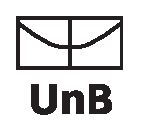
\includegraphics[width=1.5cm]{_extensions/nrennie/PrettyPDF/logo.eps}
          }%
     }%
}

%% Style the page number
\fancypagestyle{mystyle}{
  \fancyhf{}
  \renewcommand\headrulewidth{0pt}
  \fancyfoot[R]{\thepage}
  \fancyfootoffset{3.5cm}
}
\setlength{\footskip}{20pt}

%% style the chapter/section fonts
\chapterfont{\color{dark}\fontsize{20}{16.8}\selectfont}
\sectionfont{\color{dark}\fontsize{20}{16.8}\selectfont}
\subsectionfont{\color{dark}\fontsize{14}{16.8}\selectfont}
\titleformat{\subsection}
  {\sffamily\Large\bfseries}{\thesection}{1em}{}[{\titlerule[0.8pt]}]
  
% left align title
\makeatletter
\renewcommand{\maketitle}{\bgroup\setlength{\parindent}{0pt}
\begin{flushleft}
  {\sffamily\huge\textbf{\MakeUppercase{\@title}}} \vspace{1cm} \newline
  {\Large {\@subtitle}} \vspace{1cm} \newline
  \@author \newline
\end{flushleft}\egroup
}
\makeatother

%% Use some custom fonts
\setsansfont{Ubuntu}[
    Path=_extensions/nrennie/PrettyPDF/Ubuntu/,
    Scale=0.9,
    Extension = .ttf,
    UprightFont=*-Regular,
    BoldFont=*-Bold,
    ItalicFont=*-Italic,
    ]

\setmainfont{Ubuntu}[
    Path=_extensions/nrennie/PrettyPDF/Ubuntu/,
    Scale=0.9,
    Extension = .ttf,
    UprightFont=*-Regular,
    BoldFont=*-Bold,
    ItalicFont=*-Italic,
    ]
\KOMAoption{captions}{tableheading}
\makeatletter
\makeatother
\makeatletter
\@ifpackageloaded{bookmark}{}{\usepackage{bookmark}}
\makeatother
\makeatletter
\@ifpackageloaded{caption}{}{\usepackage{caption}}
\AtBeginDocument{%
\ifdefined\contentsname
  \renewcommand*\contentsname{Table of contents}
\else
  \newcommand\contentsname{Table of contents}
\fi
\ifdefined\listfigurename
  \renewcommand*\listfigurename{List of Figures}
\else
  \newcommand\listfigurename{List of Figures}
\fi
\ifdefined\listtablename
  \renewcommand*\listtablename{List of Tables}
\else
  \newcommand\listtablename{List of Tables}
\fi
\ifdefined\figurename
  \renewcommand*\figurename{Figure}
\else
  \newcommand\figurename{Figure}
\fi
\ifdefined\tablename
  \renewcommand*\tablename{Table}
\else
  \newcommand\tablename{Table}
\fi
}
\@ifpackageloaded{float}{}{\usepackage{float}}
\floatstyle{ruled}
\@ifundefined{c@chapter}{\newfloat{codelisting}{h}{lop}}{\newfloat{codelisting}{h}{lop}[chapter]}
\floatname{codelisting}{Listing}
\newcommand*\listoflistings{\listof{codelisting}{List of Listings}}
\makeatother
\makeatletter
\@ifpackageloaded{caption}{}{\usepackage{caption}}
\@ifpackageloaded{subcaption}{}{\usepackage{subcaption}}
\makeatother
\makeatletter
\@ifpackageloaded{tcolorbox}{}{\usepackage[skins,breakable]{tcolorbox}}
\makeatother
\makeatletter
\@ifundefined{shadecolor}{\definecolor{shadecolor}{rgb}{.97, .97, .97}}
\makeatother
\makeatletter
\@ifundefined{codebgcolor}{\definecolor{codebgcolor}{named}{light}}
\makeatother
\makeatletter
\makeatother
\ifLuaTeX
  \usepackage{selnolig}  % disable illegal ligatures
\fi
\IfFileExists{bookmark.sty}{\usepackage{bookmark}}{\usepackage{hyperref}}
\IfFileExists{xurl.sty}{\usepackage{xurl}}{} % add URL line breaks if available
\urlstyle{same} % disable monospaced font for URLs
\hypersetup{
  pdftitle={Prova 2 de Processo Estocásticos},
  pdfauthor={Professor Felipe Quintino},
  colorlinks=true,
  linkcolor={highlight},
  filecolor={Maroon},
  citecolor={Blue},
  urlcolor={highlight},
  pdfcreator={LaTeX via pandoc}}

\title{Prova 2 de Processo Estocásticos}
\usepackage{etoolbox}
\makeatletter
\providecommand{\subtitle}[1]{% add subtitle to \maketitle
  \apptocmd{\@title}{\par {\large #1 \par}}{}{}
}
\makeatother
\subtitle{Rafael de Acypreste (200060023) e Rafael Lira (190115858)}
\author{Professor Felipe Quintino}
\date{}

\begin{document}
\maketitle
\pagestyle{mystyle}

\ifdefined\Shaded\renewenvironment{Shaded}{\begin{tcolorbox}[borderline west={3pt}{0pt}{shadecolor}, boxrule=0pt, frame hidden, sharp corners, colback={codebgcolor}, enhanced, breakable]}{\end{tcolorbox}}\fi

\bookmarksetup{startatroot}

\hypertarget{questuxe3o-1}{%
\chapter*{Questão 1}\label{questuxe3o-1}}
\addcontentsline{toc}{chapter}{Questão 1}

\markboth{Questão 1}{Questão 1}

\hypertarget{aplicauxe7uxe3o-ao-modelo-empuxedrico}{%
\section*{Aplicação ao modelo
empírico}\label{aplicauxe7uxe3o-ao-modelo-empuxedrico}}
\addcontentsline{toc}{section}{Aplicação ao modelo empírico}

\markright{Aplicação ao modelo empírico}

Trata-se de um modelo para avaliar as probabilidades de transição entre
os estados de precipitação de chuvas.

\begin{Shaded}
\begin{Highlighting}[]
\CommentTok{\# Importing data}
\NormalTok{dados }\OtherTok{\textless{}{-}}
    \FunctionTok{read.delim}\NormalTok{(}\StringTok{"dados.txt"}\NormalTok{,}
        \AttributeTok{header =} \ConstantTok{TRUE}\NormalTok{,}
        \AttributeTok{sep    =} \StringTok{";"}
\NormalTok{    ) }\SpecialCharTok{|\textgreater{}}
    \FunctionTok{select}\NormalTok{(}\SpecialCharTok{{-}}\NormalTok{X) }\SpecialCharTok{|\textgreater{}}
    \FunctionTok{filter}\NormalTok{(}\SpecialCharTok{!}\FunctionTok{is.na}\NormalTok{(Precipitacao))}

\CommentTok{\# Summary statistics}
\NormalTok{dados}\SpecialCharTok{$}\NormalTok{Precipitacao }\SpecialCharTok{|\textgreater{}} \FunctionTok{summary}\NormalTok{()}
\end{Highlighting}
\end{Shaded}

\begin{verbatim}
   Min. 1st Qu.  Median    Mean 3rd Qu.    Max. 
  0.000   0.000   0.000   4.173   2.400 131.000 
\end{verbatim}

\begin{Shaded}
\begin{Highlighting}[]
\FunctionTok{hist}\NormalTok{(dados}\SpecialCharTok{$}\NormalTok{Precipitacao)}
\end{Highlighting}
\end{Shaded}

\begin{figure}[H]

{\centering 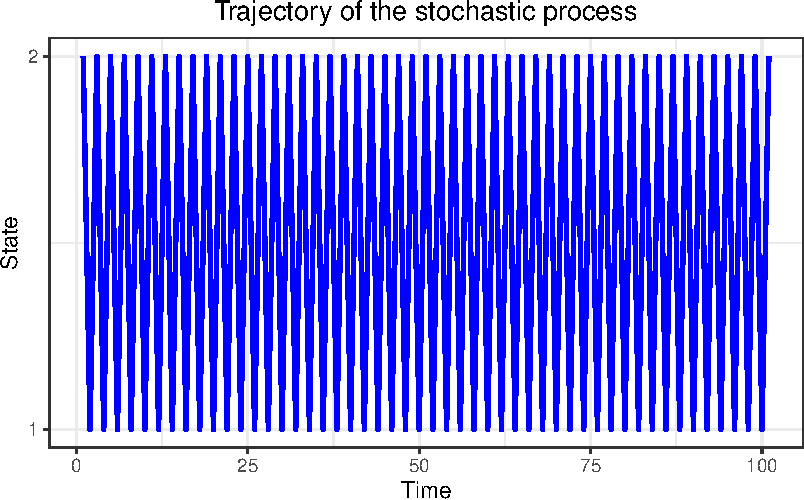
\includegraphics{index_files/figure-pdf/unnamed-chunk-2-1.pdf}

}

\end{figure}

\hypertarget{a}{%
\section*{a)}\label{a}}
\addcontentsline{toc}{section}{a)}

\markright{a)}

O primeiro passo é discretizar a variável de precipitação, que é feita
com a função \texttt{cut()} do pacote \texttt{base}. Para esse exemplo,
a variável será dividida em 5 categorias: sem chuva (precipitação até
\(0,001\)), garoa (precipitação até \(1\)), chuva fraca (precipitação
até \(4,8\)), chuva moderada (precipitação até \(14,2\)) e chuva forte
(precipitação acima de \(14,2\)).

\begin{Shaded}
\begin{Highlighting}[]
\CommentTok{\# Discretization of the variable}
\NormalTok{quantiles }\OtherTok{\textless{}{-}} \FunctionTok{quantile}\NormalTok{(dados}\SpecialCharTok{$}\NormalTok{Precipitacao,}
    \AttributeTok{probs =} \FunctionTok{seq}\NormalTok{(}\FloatTok{0.7}\NormalTok{, }\FloatTok{0.9}\NormalTok{, }\AttributeTok{length.out =} \DecValTok{3}\NormalTok{)}
\NormalTok{)}

\NormalTok{breaks }\OtherTok{\textless{}{-}} \FunctionTok{c}\NormalTok{(}\SpecialCharTok{{-}}\ConstantTok{Inf}\NormalTok{, }\FloatTok{0.001}\NormalTok{, quantiles, }\ConstantTok{Inf}\NormalTok{)}

\NormalTok{state\_labels }\OtherTok{\textless{}{-}} \FunctionTok{factor}\NormalTok{(}
    \FunctionTok{c}\NormalTok{(}
        \StringTok{"sem chuva"}\NormalTok{,}
        \StringTok{"garoa"}\NormalTok{,}
        \StringTok{"chuva fraca"}\NormalTok{,}
        \StringTok{"chuva moderada"}\NormalTok{,}
        \StringTok{"chuva forte"}
\NormalTok{    ),}
    \AttributeTok{levels =} \FunctionTok{c}\NormalTok{(}
        \StringTok{"sem chuva"}\NormalTok{,}
        \StringTok{"garoa"}\NormalTok{,}
        \StringTok{"chuva fraca"}\NormalTok{,}
        \StringTok{"chuva moderada"}\NormalTok{,}
        \StringTok{"chuva forte"}
\NormalTok{    )}
\NormalTok{)}

\CommentTok{\# Discretization}
\NormalTok{dados }\OtherTok{\textless{}{-}}
\NormalTok{    dados }\SpecialCharTok{|\textgreater{}}
    \CommentTok{\# Discretization}
    \FunctionTok{mutate}\NormalTok{(}\AttributeTok{rain\_status =} \FunctionTok{cut}\NormalTok{(Precipitacao,}
        \AttributeTok{breaks =}\NormalTok{ breaks,}
        \AttributeTok{labels =}\NormalTok{ state\_labels}
\NormalTok{    ))}
\end{Highlighting}
\end{Shaded}

\hypertarget{b}{%
\section*{b)}\label{b}}
\addcontentsline{toc}{section}{b)}

\markright{b)}

Para esse exemplo, serão separadas as 10 últimas observações para
avaliar as estimações.

\begin{Shaded}
\begin{Highlighting}[]
\NormalTok{dados\_teste }\OtherTok{\textless{}{-}} \FunctionTok{tail}\NormalTok{(dados, }\DecValTok{10}\NormalTok{)}
\NormalTok{dados\_treinamento }\OtherTok{\textless{}{-}}\NormalTok{ dados[}\DecValTok{1}\SpecialCharTok{:}\NormalTok{(}\FunctionTok{nrow}\NormalTok{(dados) }\SpecialCharTok{{-}} \DecValTok{10}\NormalTok{), ]}
\end{Highlighting}
\end{Shaded}

Para estimar as transições de estado, é necessário criar uma variável
que identifique o estado atual e o estado seguinte. Para isso, é
necessário criar uma variável defasada, que pode ser feita com a função
\texttt{lag()} do pacote \texttt{dplyr}. Depois disso, basta avaliar as
proporções das transições de estado.

\begin{Shaded}
\begin{Highlighting}[]
\CommentTok{\# Creating the lagged variable}
\NormalTok{transicoes\_chuva }\OtherTok{\textless{}{-}}
\NormalTok{    dados\_treinamento }\SpecialCharTok{|\textgreater{}}
    \CommentTok{\# Lag variable}
    \FunctionTok{mutate}\NormalTok{(}\AttributeTok{rain\_status\_lag =} \FunctionTok{lag}\NormalTok{(rain\_status)) }\SpecialCharTok{|\textgreater{}}
    \CommentTok{\# Exclude the last state}
    \FunctionTok{filter}\NormalTok{(}\SpecialCharTok{!}\FunctionTok{is.na}\NormalTok{(rain\_status\_lag)) }\SpecialCharTok{|\textgreater{}}
    \CommentTok{\# Count the transitions}
    \FunctionTok{count}\NormalTok{(rain\_status, rain\_status\_lag) }\SpecialCharTok{|\textgreater{}}
    \CommentTok{\# Calculates the estimator}
    \FunctionTok{mutate}\NormalTok{(}
        \AttributeTok{Prop =} \FunctionTok{round}\NormalTok{(n }\SpecialCharTok{/} \FunctionTok{sum}\NormalTok{(n), }\AttributeTok{digits =} \DecValTok{3}\NormalTok{),}
        \AttributeTok{.by =}\NormalTok{ rain\_status}
\NormalTok{    )}
\end{Highlighting}
\end{Shaded}

A matriz de transição estimada entre os estados sem chuva, garoa, chuva
fraca, chuva moderada, chuva forte, nesta ordem, é dada por:

\begin{equation}
P =
\begin{pmatrix}
0.822 & 0.041 &  0.051 & 0.045 &  0.04 \\
0.334 & 0.12 &  0.186 & 0.177 &  0.183 \\
0.306 & 0.133 &  0.187 & 0.184 &  0.19 \\
0.306 & 0.121 &  0.171 & 0.193 &  0.21 \\
0.282 & 0.118 &  0.174 & 0.204 &  0.223 
\end{pmatrix}
\end{equation}

Agora, pode-se recuperar a matriz de transição para fazer as estimativas
de transição de estado.

\begin{Shaded}
\begin{Highlighting}[]
\CommentTok{\# Transition matrix}
\NormalTok{matriz\_transicao }\OtherTok{\textless{}{-}}
\NormalTok{    transicoes\_chuva }\SpecialCharTok{|\textgreater{}}
    \FunctionTok{select}\NormalTok{(}\SpecialCharTok{{-}}\NormalTok{n) }\SpecialCharTok{|\textgreater{}}
    \FunctionTok{pivot\_wider}\NormalTok{(}
        \AttributeTok{names\_from =}\NormalTok{ rain\_status\_lag,}
        \AttributeTok{values\_from =}\NormalTok{ Prop}
\NormalTok{    ) }\SpecialCharTok{|\textgreater{}}
    \FunctionTok{column\_to\_rownames}\NormalTok{(}\StringTok{"rain\_status"}\NormalTok{) }\SpecialCharTok{|\textgreater{}}
    \FunctionTok{as.matrix}\NormalTok{()}

\NormalTok{matriz\_transicao}
\end{Highlighting}
\end{Shaded}

\begin{verbatim}
               sem chuva garoa chuva fraca chuva moderada chuva forte
sem chuva          0.822 0.041       0.051          0.045       0.040
garoa              0.334 0.120       0.186          0.177       0.183
chuva fraca        0.306 0.133       0.187          0.184       0.190
chuva moderada     0.306 0.121       0.171          0.193       0.210
chuva forte        0.282 0.118       0.174          0.204       0.223
\end{verbatim}

\begin{Shaded}
\begin{Highlighting}[]
\NormalTok{ultimo\_estado }\OtherTok{\textless{}{-}}\NormalTok{ dados\_treinamento }\SpecialCharTok{|\textgreater{}}
    \FunctionTok{tail}\NormalTok{(}\DecValTok{1}\NormalTok{) }\SpecialCharTok{|\textgreater{}}
    \FunctionTok{pull}\NormalTok{(rain\_status)}

\NormalTok{ultimo\_estado}
\end{Highlighting}
\end{Shaded}

\begin{verbatim}
[1] garoa
Levels: sem chuva garoa chuva fraca chuva moderada chuva forte
\end{verbatim}

\hypertarget{c}{%
\section*{c)}\label{c}}
\addcontentsline{toc}{section}{c)}

\markright{c)}

Com a matriz de transição, basta considerar o último estado dos dados de
treinamento (garoa) ---- consequência da propriedade de Markov ---- para
fazer as estimativas de transição de estado.

\begin{Shaded}
\begin{Highlighting}[]
\NormalTok{simula\_cadeia\_markov }\OtherTok{\textless{}{-}} \ControlFlowTok{function}\NormalTok{(}\AttributeTok{n =} \DecValTok{10}\NormalTok{,}
\NormalTok{                                 valor\_inicial,}
\NormalTok{                                 matriz\_transicao,}
\NormalTok{                                 estados) \{}
\NormalTok{    P }\OtherTok{\textless{}{-}}\NormalTok{ matriz\_transicao}
\NormalTok{    y }\OtherTok{\textless{}{-}}\NormalTok{ valor\_inicial}

    \CommentTok{\# Simulation of the stochastic process}
    \ControlFlowTok{for}\NormalTok{ (i }\ControlFlowTok{in} \DecValTok{1}\SpecialCharTok{:}\NormalTok{n) \{}
        \CommentTok{\# Sample of the next state}
\NormalTok{        y[i }\SpecialCharTok{+} \DecValTok{1}\NormalTok{] }\OtherTok{\textless{}{-}} \FunctionTok{sample}\NormalTok{(estados, }\AttributeTok{size =} \DecValTok{1}\NormalTok{, }\AttributeTok{prob =}\NormalTok{ P[y[i], ])}
\NormalTok{    \}}

    \FunctionTok{return}\NormalTok{(y[}\SpecialCharTok{{-}}\DecValTok{1}\NormalTok{])}
\NormalTok{\}}
\CommentTok{\# Excecution of the function}
\NormalTok{previsoes }\OtherTok{\textless{}{-}} \FunctionTok{simula\_cadeia\_markov}\NormalTok{(}
    \AttributeTok{valor\_inicial    =}\NormalTok{ ultimo\_estado,}
    \AttributeTok{matriz\_transicao =}\NormalTok{ matriz\_transicao,}
    \AttributeTok{estados          =}\NormalTok{ state\_labels,}
    \AttributeTok{n                =} \DecValTok{10}
\NormalTok{)}
\end{Highlighting}
\end{Shaded}

E, então, pode-se comparar as previsões com os dados de teste. Para o
gráfico, os acertos são indicados pela linha tracejada vermelha.

\begin{Shaded}
\begin{Highlighting}[]
\NormalTok{comparacao }\OtherTok{\textless{}{-}}
    \FunctionTok{data.frame}\NormalTok{(}
        \AttributeTok{observado =}\NormalTok{ dados\_teste}\SpecialCharTok{$}\NormalTok{rain\_status,}
        \AttributeTok{previsao =}\NormalTok{ previsoes}
\NormalTok{    )}

\CommentTok{\# Imprime a tabela}
\NormalTok{comparacao}
\end{Highlighting}
\end{Shaded}

\begin{verbatim}
        observado       previsao
1  chuva moderada chuva moderada
2  chuva moderada    chuva fraca
3     chuva forte chuva moderada
4       sem chuva          garoa
5       sem chuva    chuva fraca
6       sem chuva      sem chuva
7       sem chuva      sem chuva
8       sem chuva      sem chuva
9     chuva fraca      sem chuva
10          garoa    chuva forte
\end{verbatim}

\begin{Shaded}
\begin{Highlighting}[]
\CommentTok{\# Constroi o gráfico}
\NormalTok{comparacao }\SpecialCharTok{|\textgreater{}}
    \FunctionTok{ggplot}\NormalTok{(}\FunctionTok{aes}\NormalTok{(}\AttributeTok{x =}\NormalTok{ observado, }\AttributeTok{y =}\NormalTok{ previsao)) }\SpecialCharTok{+}
    \FunctionTok{geom\_jitter}\NormalTok{(}
        \AttributeTok{size =} \DecValTok{3}\NormalTok{, }\AttributeTok{shape =} \DecValTok{2}\NormalTok{,}
        \AttributeTok{width =} \FloatTok{0.15}\NormalTok{, }\AttributeTok{height =} \FloatTok{0.15}
\NormalTok{    ) }\SpecialCharTok{+}
    \FunctionTok{geom\_abline}\NormalTok{(}
        \AttributeTok{intercept =} \DecValTok{0}\NormalTok{,}
        \AttributeTok{slope =} \DecValTok{1}\NormalTok{,}
        \AttributeTok{color =} \StringTok{"red"}\NormalTok{,}
        \AttributeTok{linetype =} \StringTok{"dashed"}
\NormalTok{    ) }\SpecialCharTok{+}
    \FunctionTok{theme\_bw}\NormalTok{() }\SpecialCharTok{+}
    \FunctionTok{labs}\NormalTok{(}
        \AttributeTok{x =} \StringTok{"Observado"}\NormalTok{,}
        \AttributeTok{y =} \StringTok{"Previsão"}\NormalTok{,}
        \AttributeTok{title =} \StringTok{"Previsões vs. Observações"}
\NormalTok{    )}
\end{Highlighting}
\end{Shaded}

\begin{figure}[H]

{\centering 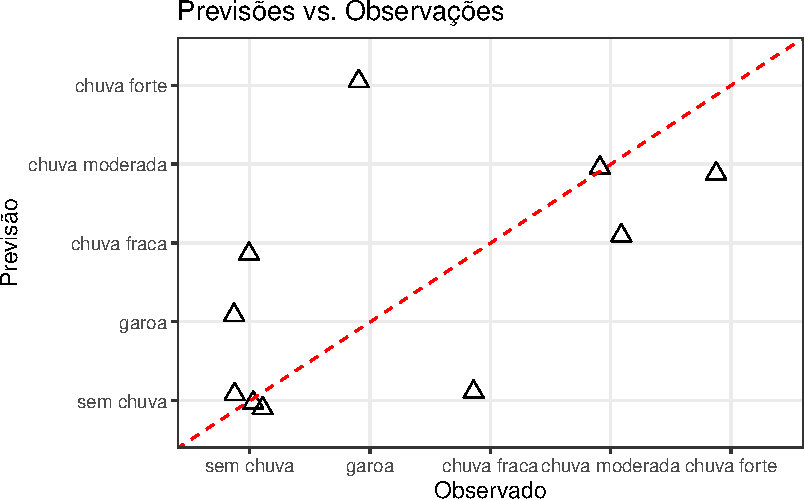
\includegraphics{index_files/figure-pdf/unnamed-chunk-8-1.pdf}

}

\end{figure}

\bookmarksetup{startatroot}

\hypertarget{questuxe3o-2}{%
\chapter*{Questão 2}\label{questuxe3o-2}}
\addcontentsline{toc}{chapter}{Questão 2}

\markboth{Questão 2}{Questão 2}

\hypertarget{aplicauxe7uxe3o-ao-modelo-empuxedrico-1}{%
\section*{Aplicação ao modelo
empírico}\label{aplicauxe7uxe3o-ao-modelo-empuxedrico-1}}
\addcontentsline{toc}{section}{Aplicação ao modelo empírico}

\markright{Aplicação ao modelo empírico}

Trata-se de um modelo para avaliar o comportamento dos preços de
fechamentos dos valores das ações do BBAS3 no ano de 2023.

\begin{Shaded}
\begin{Highlighting}[]
\CommentTok{\# Define the stock symbol and specify the start and end dates}
\NormalTok{stock\_symbol }\OtherTok{\textless{}{-}} \StringTok{"BBAS3.SA"}
\NormalTok{start\_date }\OtherTok{\textless{}{-}} \StringTok{"2023{-}01{-}01"}
\NormalTok{end\_date }\OtherTok{\textless{}{-}} \StringTok{"2024{-}01{-}01"}

\CommentTok{\# Use getSymbols to fetch historical stock data}
\FunctionTok{getSymbols}\NormalTok{(stock\_symbol,}
    \AttributeTok{src =} \StringTok{"yahoo"}\NormalTok{,}
    \AttributeTok{from =}\NormalTok{ start\_date,}
    \AttributeTok{to =}\NormalTok{ end\_date}
\NormalTok{)}
\end{Highlighting}
\end{Shaded}

\begin{verbatim}
[1] "BBAS3.SA"
\end{verbatim}

\begin{Shaded}
\begin{Highlighting}[]
\CommentTok{\# Check the loaded data and get the closing values}
\NormalTok{stock\_values }\OtherTok{\textless{}{-}} \FunctionTok{as.vector}\NormalTok{(}\FunctionTok{Cl}\NormalTok{(}\FunctionTok{get}\NormalTok{(stock\_symbol)))}

\CommentTok{\# Summary statistics}
\FunctionTok{summary}\NormalTok{(stock\_values)}
\end{Highlighting}
\end{Shaded}

\begin{verbatim}
   Min. 1st Qu.  Median    Mean 3rd Qu.    Max. 
  32.64   40.78   47.00   45.49   49.07   55.39 
\end{verbatim}

\hypertarget{a-1}{%
\section*{a)}\label{a-1}}
\addcontentsline{toc}{section}{a)}

\markright{a)}

Obtendo o número de observações no vetor de valores da ação, é possível
gerar simulações do movimento Browniano e do processo de Poisson (padrão
e compensado) com a mesma quantidade de pontos que a base de dados.
Considerando um intervalo de 0 a 1, em anos, é gerado um vetor \(t\)
relativo ao tempo decorrido do início da contagem ao momento de cada
observação.

Para simular o movimento Browniano, basta fazer a soma cumulativa de
\(n\) valores da distribuição Normal padrão. Para o processo de Poisson
é feita a soma de valores da distribuição Poisson com parâmetro
\(\lambda=1\). Por fim, para o processo de Poisson compensado, é feita a
soma de valores da distribuição Poisson com parâmetro \(\lambda=1\)
subtraídos de \(\lambda t_{k} = t_{k}\), onde \(t_{k}\) é o tempo
decorrido do início da contagem ao momento de cada observação.

\begin{Shaded}
\begin{Highlighting}[]
\NormalTok{n }\OtherTok{\textless{}{-}} \FunctionTok{length}\NormalTok{(stock\_values) }\SpecialCharTok{{-}} \DecValTok{1}
\NormalTok{t }\OtherTok{\textless{}{-}} \FunctionTok{seq}\NormalTok{(}\DecValTok{0}\NormalTok{, }\DecValTok{1}\NormalTok{, }\AttributeTok{length.out =}\NormalTok{ n }\SpecialCharTok{+} \DecValTok{1}\NormalTok{)}
\NormalTok{B }\OtherTok{\textless{}{-}} \FunctionTok{c}\NormalTok{(}\DecValTok{0}\NormalTok{, }\FunctionTok{cumsum}\NormalTok{(}\FunctionTok{rnorm}\NormalTok{(n, }\AttributeTok{mean =} \DecValTok{0}\NormalTok{, }\AttributeTok{sd =} \DecValTok{1}\NormalTok{)))}
\NormalTok{N }\OtherTok{\textless{}{-}} \FunctionTok{c}\NormalTok{(}\DecValTok{0}\NormalTok{, }\FunctionTok{cumsum}\NormalTok{(}\FunctionTok{rpois}\NormalTok{(n, }\AttributeTok{lambda =} \DecValTok{1}\NormalTok{)))}
\NormalTok{N\_compensated }\OtherTok{\textless{}{-}} \FunctionTok{c}\NormalTok{(}\DecValTok{0}\NormalTok{, }\FunctionTok{cumsum}\NormalTok{(}\FunctionTok{rpois}\NormalTok{(n, }\AttributeTok{lambda =} \DecValTok{1}\NormalTok{)) }\SpecialCharTok{{-}} \FunctionTok{seq}\NormalTok{(}\DecValTok{1}\NormalTok{, n, }\AttributeTok{by =} \DecValTok{1}\NormalTok{))}
\end{Highlighting}
\end{Shaded}

\begin{Shaded}
\begin{Highlighting}[]
\FunctionTok{data.frame}\NormalTok{(}\AttributeTok{time =}\NormalTok{ t, }\AttributeTok{Browniano =}\NormalTok{ B) }\SpecialCharTok{|\textgreater{}} 
    \FunctionTok{ggplot}\NormalTok{(}\FunctionTok{aes}\NormalTok{(}\AttributeTok{x =}\NormalTok{ time, }\AttributeTok{y =}\NormalTok{ Browniano)) }\SpecialCharTok{+}
    \FunctionTok{geom\_line}\NormalTok{(}\AttributeTok{color =} \StringTok{"lightblue"}\NormalTok{) }\SpecialCharTok{+}
    \FunctionTok{labs}\NormalTok{(}
        \AttributeTok{x =} \StringTok{"Tempo"}\NormalTok{,}
        \AttributeTok{y =} \StringTok{"Valor do movimento Browniano"}\NormalTok{,}
        \AttributeTok{title =} \StringTok{"Simulação do movimento Browniano"}
\NormalTok{    ) }\SpecialCharTok{+}
    \FunctionTok{theme\_minimal}\NormalTok{()}
\end{Highlighting}
\end{Shaded}

\begin{figure}[H]

{\centering 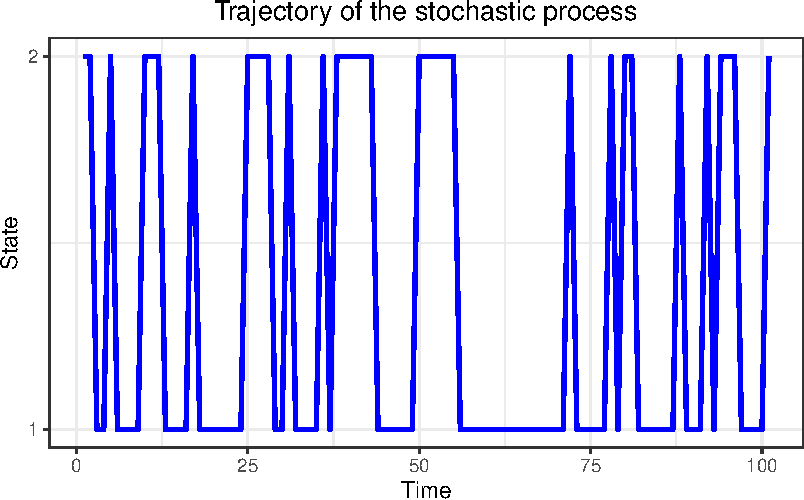
\includegraphics{questao-2_files/figure-pdf/unnamed-chunk-4-1.pdf}

}

\end{figure}

\begin{Shaded}
\begin{Highlighting}[]
\FunctionTok{data.frame}\NormalTok{(}\AttributeTok{time =}\NormalTok{ t, }\AttributeTok{Poisson =}\NormalTok{ N) }\SpecialCharTok{|\textgreater{}} 
    \FunctionTok{ggplot}\NormalTok{(}\FunctionTok{aes}\NormalTok{(}\AttributeTok{x =}\NormalTok{ time, }\AttributeTok{y =}\NormalTok{ Poisson)) }\SpecialCharTok{+}
    \FunctionTok{geom\_step}\NormalTok{(}\AttributeTok{color =} \StringTok{"darkred"}\NormalTok{) }\SpecialCharTok{+}
    \FunctionTok{labs}\NormalTok{(}
        \AttributeTok{x =} \StringTok{"Tempo"}\NormalTok{,}
        \AttributeTok{y =} \StringTok{"Valor do processo de Poisson"}\NormalTok{,}
        \AttributeTok{title =} \StringTok{"Simulação do processo de Poisson"}
\NormalTok{    ) }\SpecialCharTok{+}
    \FunctionTok{theme\_minimal}\NormalTok{()}
\end{Highlighting}
\end{Shaded}

\begin{figure}[H]

{\centering 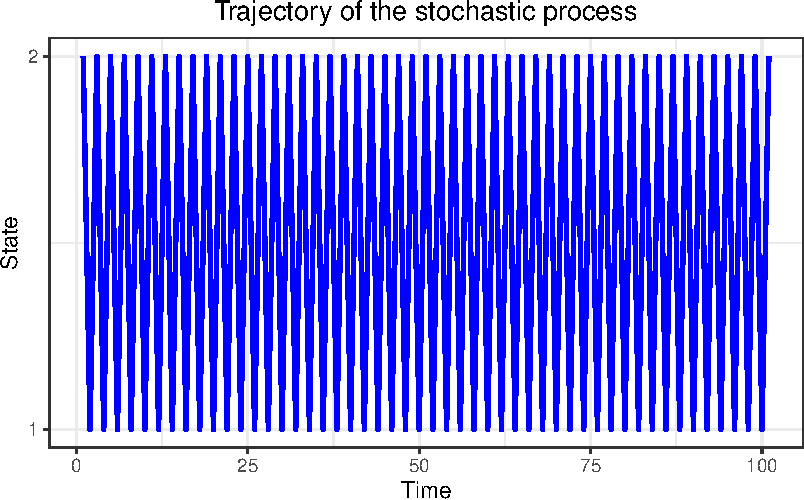
\includegraphics{questao-2_files/figure-pdf/unnamed-chunk-5-1.pdf}

}

\end{figure}

\begin{Shaded}
\begin{Highlighting}[]
\FunctionTok{data.frame}\NormalTok{(}\AttributeTok{time =}\NormalTok{ t, }\AttributeTok{Compensated =}\NormalTok{ N\_compensated) }\SpecialCharTok{|\textgreater{}} 
    \FunctionTok{ggplot}\NormalTok{(}\FunctionTok{aes}\NormalTok{(}\AttributeTok{x =}\NormalTok{ time, }\AttributeTok{y =}\NormalTok{ Compensated)) }\SpecialCharTok{+}
    \FunctionTok{geom\_step}\NormalTok{(}\AttributeTok{color =} \StringTok{"darkred"}\NormalTok{) }\SpecialCharTok{+}
    \FunctionTok{labs}\NormalTok{(}
        \AttributeTok{x =} \StringTok{"Tempo"}\NormalTok{,}
        \AttributeTok{y =} \StringTok{"Valor do processo de Poisson Compensado"}\NormalTok{,}
        \AttributeTok{title =} \StringTok{"Simulação do processo de Poisson Compensado"}
\NormalTok{    ) }\SpecialCharTok{+}
    \FunctionTok{theme\_minimal}\NormalTok{()}
\end{Highlighting}
\end{Shaded}

\begin{figure}[H]

{\centering 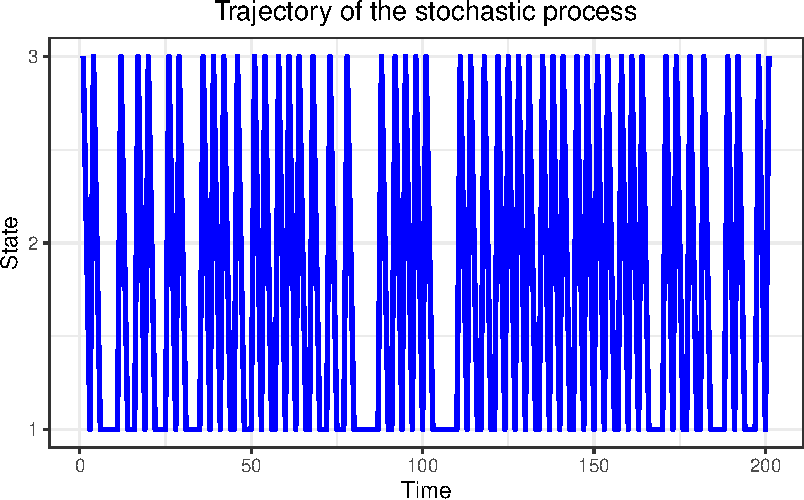
\includegraphics{questao-2_files/figure-pdf/unnamed-chunk-6-1.pdf}

}

\end{figure}

\hypertarget{b-1}{%
\section*{b)}\label{b-1}}
\addcontentsline{toc}{section}{b)}

\markright{b)}

Em seguida, é criada uma função para prever a k-ésima observação do
modelo, usando os tempos, o histórico do processo, o parâmetro
\(\theta\) e o valor do processo \(\xi(t_{k})\)

\begin{Shaded}
\begin{Highlighting}[]
\NormalTok{simulate\_Xtk }\OtherTok{\textless{}{-}} \ControlFlowTok{function}\NormalTok{(t, X, theta, csi) \{}
\NormalTok{    timeline }\OtherTok{\textless{}{-}} \FunctionTok{as.vector}\NormalTok{(t)}
\NormalTok{    history }\OtherTok{\textless{}{-}} \FunctionTok{as.vector}\NormalTok{(X)}
\NormalTok{    csi }\OtherTok{\textless{}{-}} \FunctionTok{as.vector}\NormalTok{(csi)}
\NormalTok{    stop}

    \ControlFlowTok{if}\NormalTok{ (}\FunctionTok{length}\NormalTok{(timeline) }\SpecialCharTok{!=} \FunctionTok{length}\NormalTok{(history) }\SpecialCharTok{||}
        \FunctionTok{length}\NormalTok{(timeline) }\SpecialCharTok{!=} \FunctionTok{length}\NormalTok{(csi) }\SpecialCharTok{||}
        \FunctionTok{length}\NormalTok{(history) }\SpecialCharTok{!=} \FunctionTok{length}\NormalTok{(csi)) \{}
        \FunctionTok{stop}\NormalTok{(}\StringTok{"The timeline, the history and the csi vector must have the same length!"}\NormalTok{)}
\NormalTok{    \}}

\NormalTok{    n }\OtherTok{\textless{}{-}} \FunctionTok{length}\NormalTok{(timeline)}

\NormalTok{    tj }\OtherTok{\textless{}{-}}\NormalTok{ timeline[}\SpecialCharTok{{-}}\DecValTok{1}\NormalTok{]}
\NormalTok{    tj\_1 }\OtherTok{\textless{}{-}}\NormalTok{ timeline[}\SpecialCharTok{{-}}\NormalTok{n]}
\NormalTok{    Xtj\_1 }\OtherTok{\textless{}{-}}\NormalTok{ history[}\SpecialCharTok{{-}}\NormalTok{n]}
\NormalTok{    fatork }\OtherTok{\textless{}{-}}\NormalTok{ Xtj\_1 }\SpecialCharTok{*}\NormalTok{ (tj }\SpecialCharTok{{-}}\NormalTok{ tj\_1)}
\NormalTok{    sumk }\OtherTok{\textless{}{-}} \FunctionTok{cumsum}\NormalTok{(fatork)}
\NormalTok{    Xtk }\OtherTok{\textless{}{-}}\NormalTok{ Xtj\_1 }\SpecialCharTok{{-}}\NormalTok{ theta }\SpecialCharTok{*}\NormalTok{ sumk }\SpecialCharTok{+}\NormalTok{ csi[}\SpecialCharTok{{-}}\DecValTok{1}\NormalTok{]}

    \FunctionTok{return}\NormalTok{(Xtk)}
\NormalTok{\}}
\end{Highlighting}
\end{Shaded}

\hypertarget{c-1}{%
\section*{c)}\label{c-1}}
\addcontentsline{toc}{section}{c)}

\markright{c)}

Para estimar o parâmetro \(\theta\) por meio do método dos mínimos
quadrados, é criada uma função que recebe os mesmos \emph{inputs} da
função de simulação, porém retornando a soma de quadrados do resíduo.

\begin{Shaded}
\begin{Highlighting}[]
\NormalTok{least\_squares }\OtherTok{\textless{}{-}} \ControlFlowTok{function}\NormalTok{(t, X, theta, csi) \{}
\NormalTok{    observed\_values }\OtherTok{\textless{}{-}}\NormalTok{ X[}\SpecialCharTok{{-}}\DecValTok{1}\NormalTok{]}
\NormalTok{    predicted\_values }\OtherTok{\textless{}{-}} \FunctionTok{simulate\_Xtk}\NormalTok{(t, X, theta, csi)}

    \FunctionTok{return}\NormalTok{(}\FunctionTok{sum}\NormalTok{((observed\_values }\SpecialCharTok{{-}}\NormalTok{ predicted\_values)}\SpecialCharTok{\^{}}\DecValTok{2}\NormalTok{))}
\NormalTok{\}}
\end{Highlighting}
\end{Shaded}

Utilizando a função \texttt{optim}, e escolhendo um valor inicial
inicial para \(\theta\), é possível encontrar o ponto onde a soma de
quadrados é mínima. Assim, são gerados os estimadores para cada o
movimento Browniano e para o processo de Poisson.

\begin{Shaded}
\begin{Highlighting}[]
\NormalTok{initial\_theta }\OtherTok{\textless{}{-}} \DecValTok{100}

\NormalTok{(estim\_theta\_browniano }\OtherTok{\textless{}{-}} \FunctionTok{optim}\NormalTok{(}
    \AttributeTok{par =}\NormalTok{ initial\_theta,}
    \AttributeTok{fn =}\NormalTok{ least\_squares,}
    \AttributeTok{X =}\NormalTok{ stock\_values,}
    \AttributeTok{t =}\NormalTok{ t,}
    \AttributeTok{csi =}\NormalTok{ B }\DocumentationTok{\#\# Trajetória do movimento Browniano}
\NormalTok{)}\SpecialCharTok{$}\NormalTok{par)}
\end{Highlighting}
\end{Shaded}

\begin{verbatim}
[1] 0.01953125
\end{verbatim}

\begin{Shaded}
\begin{Highlighting}[]
\NormalTok{(estim\_theta\_poisson }\OtherTok{\textless{}{-}} \FunctionTok{optim}\NormalTok{(}
    \AttributeTok{par =}\NormalTok{ initial\_theta,}
    \AttributeTok{fn =}\NormalTok{ least\_squares,}
    \AttributeTok{X =}\NormalTok{ stock\_values,}
    \AttributeTok{t =}\NormalTok{ t,}
    \AttributeTok{csi =}\NormalTok{ N }\DocumentationTok{\#\# Trajetória do processo de Poisson}
\NormalTok{)}\SpecialCharTok{$}\NormalTok{par)}
\end{Highlighting}
\end{Shaded}

\begin{verbatim}
[1] 5.9375
\end{verbatim}

\begin{Shaded}
\begin{Highlighting}[]
\NormalTok{(estim\_theta\_poisson\_compensated }\OtherTok{\textless{}{-}} \FunctionTok{optim}\NormalTok{(}
    \AttributeTok{par =}\NormalTok{ initial\_theta,}
    \AttributeTok{fn =}\NormalTok{ least\_squares,}
    \AttributeTok{X =}\NormalTok{ stock\_values,}
    \AttributeTok{t =}\NormalTok{ t,}
    \AttributeTok{csi =}\NormalTok{ N\_compensated }\DocumentationTok{\#\# Trajetória do processo de Poisson}
\NormalTok{)}\SpecialCharTok{$}\NormalTok{par)}
\end{Highlighting}
\end{Shaded}

\begin{verbatim}
[1] -0.5078125
\end{verbatim}

\hypertarget{d}{%
\section*{d)}\label{d}}
\addcontentsline{toc}{section}{d)}

\markright{d)}

Os testes dos resíduos são feitos a seguir. O que se percebe é que os
resíduos gerados pelos três modelos não seguem uma distribuição normal,
o que pode ser observado pelos valores-p do teste de Shapiro-Wilk e
pelos gráficos de histograma e de quantis.

Uma das possíveis razões pode ser a presença de autocorrelação nos
resíduos, o que é confirmado pelo gráfico de autocorrelação.

\begin{Shaded}
\begin{Highlighting}[]
\NormalTok{X\_prev\_browniano }\OtherTok{\textless{}{-}}
    \FunctionTok{simulate\_Xtk}\NormalTok{(t, stock\_values, estim\_theta\_browniano, B)}
\NormalTok{X\_prev\_poisson }\OtherTok{\textless{}{-}}
    \FunctionTok{simulate\_Xtk}\NormalTok{(t, stock\_values, estim\_theta\_poisson, N)}
\NormalTok{X\_prev\_poisson\_compensated }\OtherTok{\textless{}{-}}
    \FunctionTok{simulate\_Xtk}\NormalTok{(t, stock\_values, estim\_theta\_poisson\_compensated, N\_compensated)}

\NormalTok{residuo\_browniano }\OtherTok{\textless{}{-}}\NormalTok{ stock\_values[}\SpecialCharTok{{-}}\DecValTok{1}\NormalTok{] }\SpecialCharTok{{-}}\NormalTok{ X\_prev\_browniano}
\FunctionTok{shapiro.test}\NormalTok{(residuo\_browniano)}
\end{Highlighting}
\end{Shaded}

\begin{verbatim}

    Shapiro-Wilk normality test

data:  residuo_browniano
W = 0.97457, p-value = 0.000208
\end{verbatim}

\begin{Shaded}
\begin{Highlighting}[]
\FunctionTok{hist}\NormalTok{(residuo\_browniano)}
\end{Highlighting}
\end{Shaded}

\begin{figure}[H]

{\centering 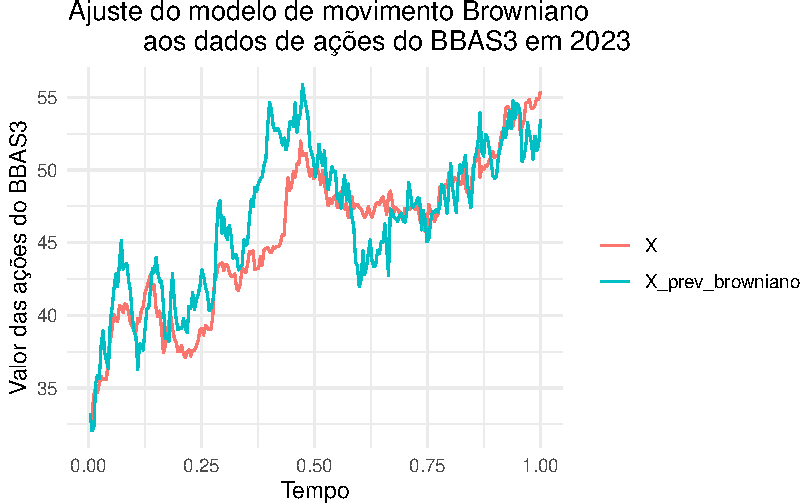
\includegraphics{questao-2_files/figure-pdf/unnamed-chunk-10-1.pdf}

}

\end{figure}

\begin{Shaded}
\begin{Highlighting}[]
\FunctionTok{qqnorm}\NormalTok{(residuo\_browniano)}
\FunctionTok{qqline}\NormalTok{(residuo\_browniano)}
\end{Highlighting}
\end{Shaded}

\begin{figure}[H]

{\centering 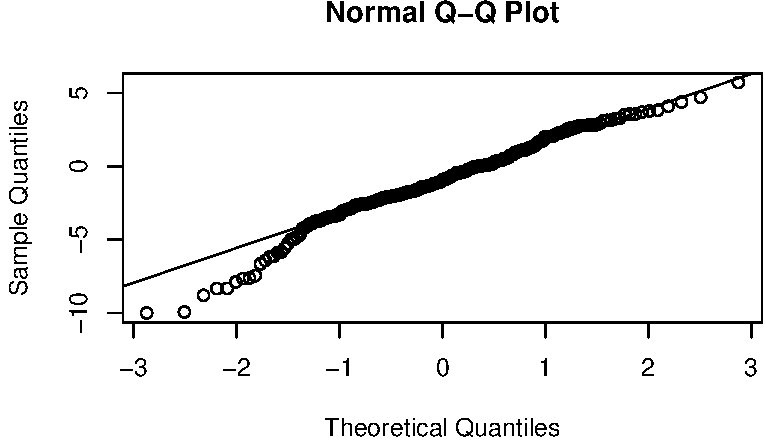
\includegraphics{questao-2_files/figure-pdf/unnamed-chunk-10-2.pdf}

}

\end{figure}

\begin{Shaded}
\begin{Highlighting}[]
\FunctionTok{acf}\NormalTok{(residuo\_browniano)}
\end{Highlighting}
\end{Shaded}

\begin{figure}[H]

{\centering 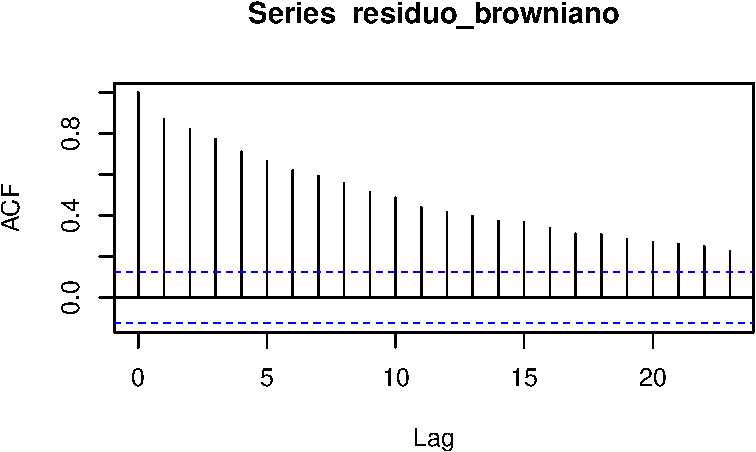
\includegraphics{questao-2_files/figure-pdf/unnamed-chunk-10-3.pdf}

}

\end{figure}

\begin{Shaded}
\begin{Highlighting}[]
\NormalTok{residuo\_poisson }\OtherTok{\textless{}{-}}\NormalTok{ stock\_values[}\SpecialCharTok{{-}}\DecValTok{1}\NormalTok{] }\SpecialCharTok{{-}}\NormalTok{ X\_prev\_poisson}
\FunctionTok{shapiro.test}\NormalTok{(residuo\_poisson)}
\end{Highlighting}
\end{Shaded}

\begin{verbatim}

    Shapiro-Wilk normality test

data:  residuo_poisson
W = 0.93173, p-value = 2.835e-09
\end{verbatim}

\begin{Shaded}
\begin{Highlighting}[]
\FunctionTok{hist}\NormalTok{(residuo\_poisson)}
\end{Highlighting}
\end{Shaded}

\begin{figure}[H]

{\centering 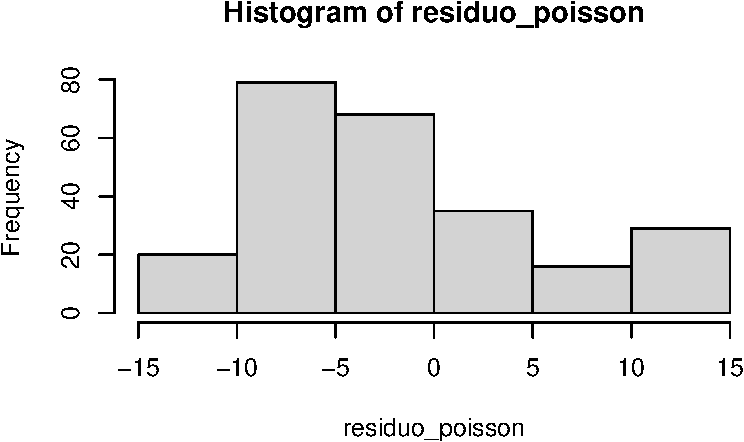
\includegraphics{questao-2_files/figure-pdf/unnamed-chunk-10-4.pdf}

}

\end{figure}

\begin{Shaded}
\begin{Highlighting}[]
\FunctionTok{qqnorm}\NormalTok{(residuo\_poisson)}
\FunctionTok{qqline}\NormalTok{(residuo\_poisson)}
\end{Highlighting}
\end{Shaded}

\begin{figure}[H]

{\centering 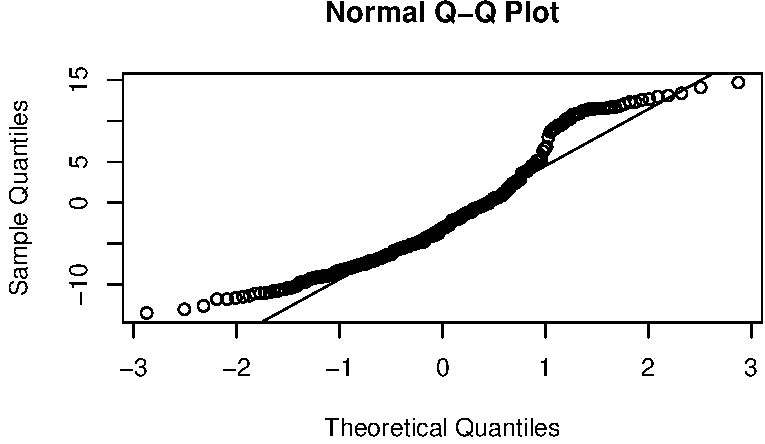
\includegraphics{questao-2_files/figure-pdf/unnamed-chunk-10-5.pdf}

}

\end{figure}

\begin{Shaded}
\begin{Highlighting}[]
\FunctionTok{acf}\NormalTok{(residuo\_poisson)}
\end{Highlighting}
\end{Shaded}

\begin{figure}[H]

{\centering 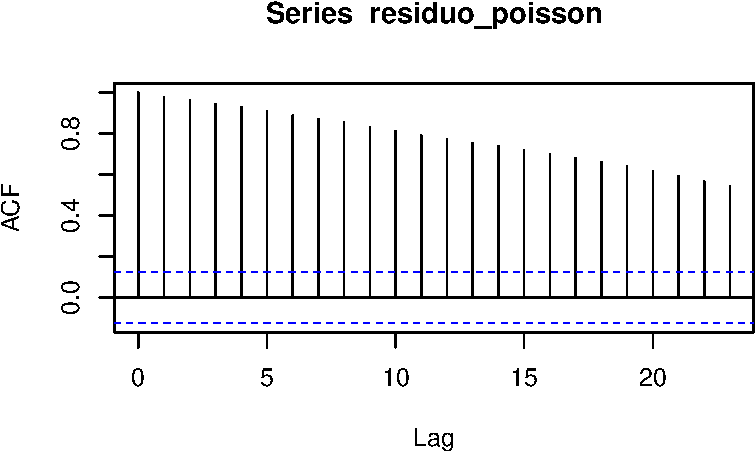
\includegraphics{questao-2_files/figure-pdf/unnamed-chunk-10-6.pdf}

}

\end{figure}

\begin{Shaded}
\begin{Highlighting}[]
\NormalTok{residuo\_poisson\_compensated }\OtherTok{\textless{}{-}}\NormalTok{ stock\_values[}\SpecialCharTok{{-}}\DecValTok{1}\NormalTok{] }\SpecialCharTok{{-}}\NormalTok{ X\_prev\_poisson\_compensated}
\FunctionTok{shapiro.test}\NormalTok{(residuo\_poisson\_compensated)}
\end{Highlighting}
\end{Shaded}

\begin{verbatim}

    Shapiro-Wilk normality test

data:  residuo_poisson_compensated
W = 0.9024, p-value = 1.395e-11
\end{verbatim}

\begin{Shaded}
\begin{Highlighting}[]
\FunctionTok{hist}\NormalTok{(residuo\_poisson\_compensated)}
\end{Highlighting}
\end{Shaded}

\begin{figure}[H]

{\centering 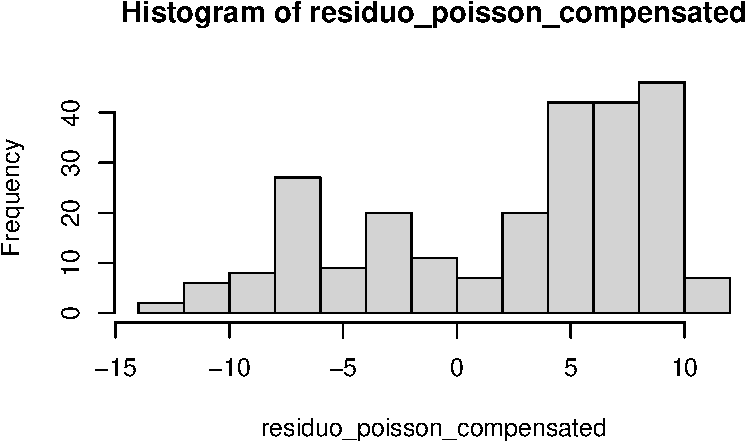
\includegraphics{questao-2_files/figure-pdf/unnamed-chunk-10-7.pdf}

}

\end{figure}

\begin{Shaded}
\begin{Highlighting}[]
\FunctionTok{qqnorm}\NormalTok{(residuo\_poisson\_compensated)}
\FunctionTok{qqline}\NormalTok{(residuo\_poisson\_compensated)}
\end{Highlighting}
\end{Shaded}

\begin{figure}[H]

{\centering 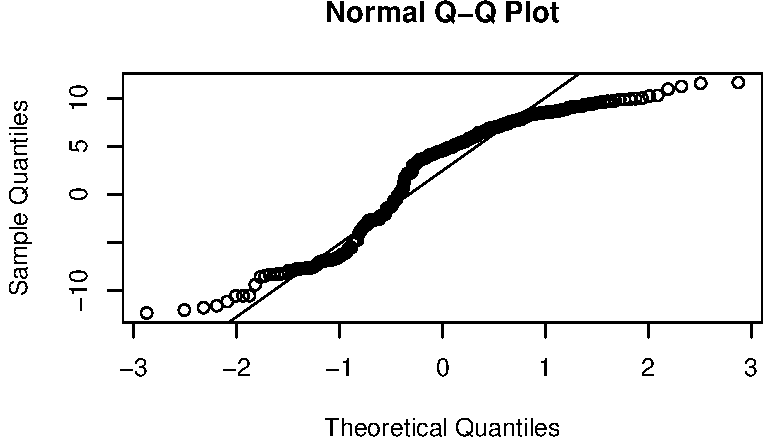
\includegraphics{questao-2_files/figure-pdf/unnamed-chunk-10-8.pdf}

}

\end{figure}

\begin{Shaded}
\begin{Highlighting}[]
\FunctionTok{acf}\NormalTok{(residuo\_poisson\_compensated)}
\end{Highlighting}
\end{Shaded}

\begin{figure}[H]

{\centering 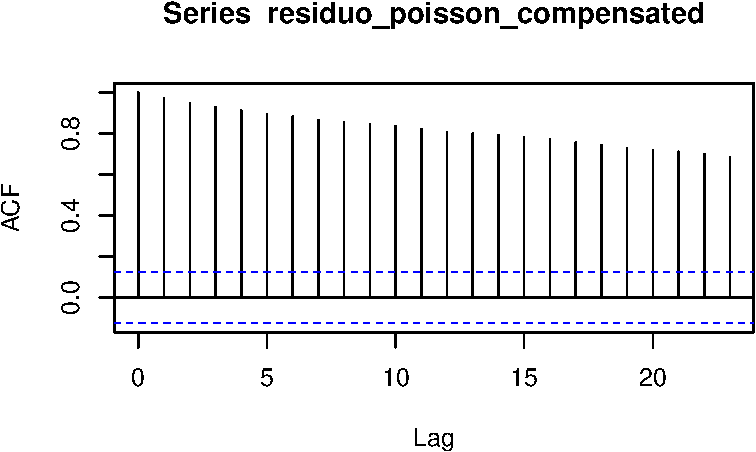
\includegraphics{questao-2_files/figure-pdf/unnamed-chunk-10-9.pdf}

}

\end{figure}

\hypertarget{e}{%
\section*{e)}\label{e}}
\addcontentsline{toc}{section}{e)}

\markright{e)}

Os modelos ajustados estão representados nos gráficos a seguir. Em todos
eles, a série original está representada em vermelho. Visualmente, o
modelo que melhor se ajusta aos dados é o modelo de movimento Browniano.
Para testar isso, são realizados testes no item f.

\begin{Shaded}
\begin{Highlighting}[]
\NormalTok{dados\_mod }\OtherTok{\textless{}{-}} \FunctionTok{data.frame}\NormalTok{(}
    \AttributeTok{t =}\NormalTok{ t[}\SpecialCharTok{{-}}\DecValTok{1}\NormalTok{],}
    \AttributeTok{X =}\NormalTok{ stock\_values[}\SpecialCharTok{{-}}\DecValTok{1}\NormalTok{],}
    \AttributeTok{X\_prev\_browniano =}\NormalTok{ X\_prev\_browniano,}
    \AttributeTok{X\_prev\_poisson =}\NormalTok{ X\_prev\_poisson,}
    \AttributeTok{X\_prev\_poisson\_compensated =}\NormalTok{ X\_prev\_poisson\_compensated}
\NormalTok{)}
\NormalTok{dados\_sim }\OtherTok{\textless{}{-}}\NormalTok{ dados\_mod }\SpecialCharTok{|\textgreater{}}
    \FunctionTok{pivot\_longer}\NormalTok{(}
        \AttributeTok{cols =} \FunctionTok{c}\NormalTok{(X,}
\NormalTok{                 X\_prev\_browniano,}
\NormalTok{                 X\_prev\_poisson,}
\NormalTok{                 X\_prev\_poisson\_compensated),}
        \AttributeTok{names\_to =} \StringTok{"Variavel"}\NormalTok{,}
        \AttributeTok{values\_to =} \StringTok{"Valor"}
\NormalTok{    )}
\end{Highlighting}
\end{Shaded}

\begin{Shaded}
\begin{Highlighting}[]
\NormalTok{dados\_sim }\SpecialCharTok{|\textgreater{}}
    \FunctionTok{filter}\NormalTok{(Variavel }\SpecialCharTok{\%in\%} \FunctionTok{c}\NormalTok{(}\StringTok{"X"}\NormalTok{, }\StringTok{"X\_prev\_browniano"}\NormalTok{)) }\SpecialCharTok{|\textgreater{}}
    \FunctionTok{ggplot}\NormalTok{() }\SpecialCharTok{+}
    \FunctionTok{geom\_line}\NormalTok{(}\FunctionTok{aes}\NormalTok{(}\AttributeTok{x =}\NormalTok{ t, }\AttributeTok{y =}\NormalTok{ Valor, }\AttributeTok{color =}\NormalTok{ Variavel)) }\SpecialCharTok{+}
    \FunctionTok{labs}\NormalTok{(}
        \AttributeTok{x =} \StringTok{"Tempo"}\NormalTok{,}
        \AttributeTok{y =} \StringTok{"Valor das ações do BBAS3"}\NormalTok{,}
        \AttributeTok{color =} \ConstantTok{NULL}\NormalTok{,}
        \AttributeTok{title =} \StringTok{"Ajuste do modelo de movimento Browniano}
\StringTok{          aos dados de ações do BBAS3 em 2023"}
\NormalTok{    ) }\SpecialCharTok{+}
    \FunctionTok{theme\_minimal}\NormalTok{()}
\end{Highlighting}
\end{Shaded}

\begin{figure}[H]

{\centering 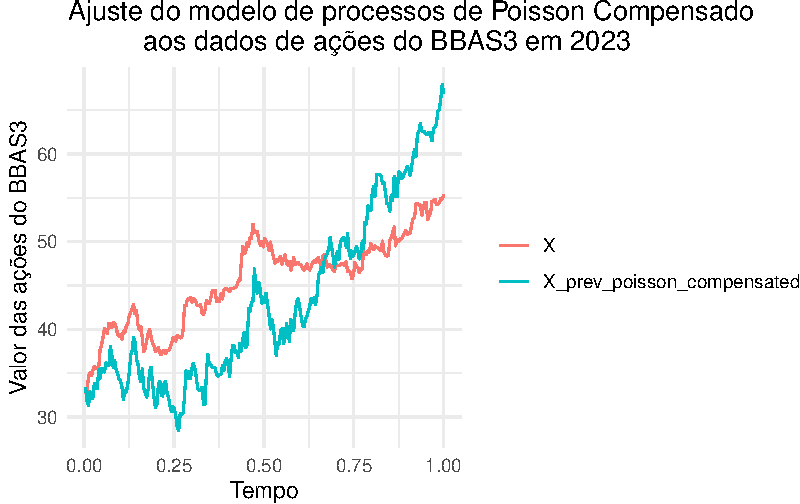
\includegraphics{questao-2_files/figure-pdf/unnamed-chunk-12-1.pdf}

}

\end{figure}

\begin{Shaded}
\begin{Highlighting}[]
\NormalTok{dados\_sim }\SpecialCharTok{|\textgreater{}}
    \FunctionTok{filter}\NormalTok{(Variavel }\SpecialCharTok{\%in\%} \FunctionTok{c}\NormalTok{(}\StringTok{"X"}\NormalTok{, }\StringTok{"X\_prev\_poisson"}\NormalTok{)) }\SpecialCharTok{|\textgreater{}}
    \FunctionTok{ggplot}\NormalTok{() }\SpecialCharTok{+}
    \FunctionTok{geom\_line}\NormalTok{(}\FunctionTok{aes}\NormalTok{(}\AttributeTok{x =}\NormalTok{ t, }\AttributeTok{y =}\NormalTok{ Valor, }\AttributeTok{color =}\NormalTok{ Variavel)) }\SpecialCharTok{+}
    \FunctionTok{labs}\NormalTok{(}
        \AttributeTok{x =} \StringTok{"Tempo"}\NormalTok{,}
        \AttributeTok{y =} \StringTok{"Valor das ações do BBAS3"}\NormalTok{,}
        \AttributeTok{color =} \ConstantTok{NULL}\NormalTok{,}
        \AttributeTok{title =} \StringTok{"Ajuste do modelo de processos de Poisson}
\StringTok{          aos dados de ações do BBAS3 em 2023"}
\NormalTok{    ) }\SpecialCharTok{+}
    \FunctionTok{theme\_minimal}\NormalTok{()}
\end{Highlighting}
\end{Shaded}

\begin{figure}[H]

{\centering 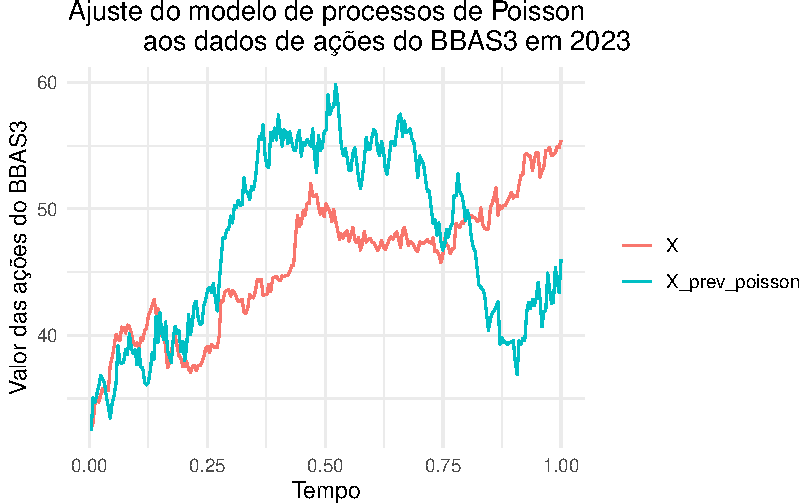
\includegraphics{questao-2_files/figure-pdf/unnamed-chunk-13-1.pdf}

}

\end{figure}

\begin{Shaded}
\begin{Highlighting}[]
\NormalTok{dados\_sim }\SpecialCharTok{|\textgreater{}}
    \FunctionTok{filter}\NormalTok{(Variavel }\SpecialCharTok{\%in\%} \FunctionTok{c}\NormalTok{(}\StringTok{"X"}\NormalTok{, }\StringTok{"X\_prev\_poisson\_compensated"}\NormalTok{)) }\SpecialCharTok{|\textgreater{}}
    \FunctionTok{ggplot}\NormalTok{() }\SpecialCharTok{+}
    \FunctionTok{geom\_line}\NormalTok{(}\FunctionTok{aes}\NormalTok{(}\AttributeTok{x =}\NormalTok{ t, }\AttributeTok{y =}\NormalTok{ Valor, }\AttributeTok{color =}\NormalTok{ Variavel)) }\SpecialCharTok{+}
    \FunctionTok{labs}\NormalTok{(}
        \AttributeTok{x =} \StringTok{"Tempo"}\NormalTok{,}
        \AttributeTok{y =} \StringTok{"Valor das ações do BBAS3"}\NormalTok{,}
        \AttributeTok{color =} \ConstantTok{NULL}\NormalTok{,}
        \AttributeTok{title =} \StringTok{"Ajuste do modelo de processos de Poisson Compensado}
\StringTok{          aos dados de ações do BBAS3 em 2023"}
\NormalTok{    ) }\SpecialCharTok{+}
    \FunctionTok{theme\_minimal}\NormalTok{()}
\end{Highlighting}
\end{Shaded}

\begin{figure}[H]

{\centering 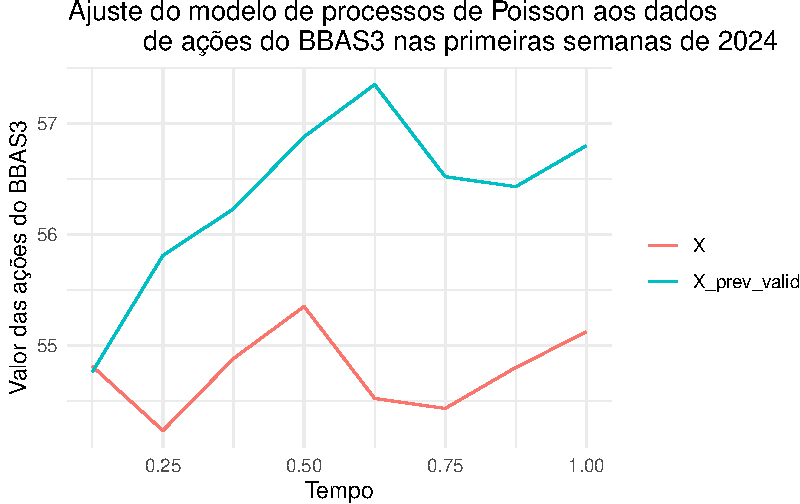
\includegraphics{questao-2_files/figure-pdf/unnamed-chunk-14-1.pdf}

}

\end{figure}

\hypertarget{f-definindo-o-melhor-modelo}{%
\section*{f) Definindo o melhor
modelo}\label{f-definindo-o-melhor-modelo}}
\addcontentsline{toc}{section}{f) Definindo o melhor modelo}

\markright{f) Definindo o melhor modelo}

Para definir o melhor modelo, pode-se comparar as métricas mais
comumento usadas:

\begin{Shaded}
\begin{Highlighting}[]
\NormalTok{mse\_browniano }\OtherTok{\textless{}{-}} \FunctionTok{mean}\NormalTok{(residuo\_browniano}\SpecialCharTok{**}\DecValTok{2}\NormalTok{)}
\NormalTok{modelo\_browniano }\OtherTok{\textless{}{-}} \FunctionTok{lm}\NormalTok{(}\AttributeTok{data =}\NormalTok{ dados\_mod, X }\SpecialCharTok{\textasciitilde{}}\NormalTok{ X\_prev\_browniano)}
\NormalTok{r2\_browniano }\OtherTok{\textless{}{-}} \FunctionTok{summary}\NormalTok{(modelo\_browniano)}\SpecialCharTok{$}\NormalTok{r.squared}
\NormalTok{aic\_browniano }\OtherTok{\textless{}{-}} \FunctionTok{AIC}\NormalTok{(modelo\_browniano)}

\NormalTok{mse\_poisson }\OtherTok{\textless{}{-}} \FunctionTok{mean}\NormalTok{(residuo\_poisson}\SpecialCharTok{**}\DecValTok{2}\NormalTok{)}
\NormalTok{modelo\_poisson }\OtherTok{\textless{}{-}} \FunctionTok{lm}\NormalTok{(}\AttributeTok{data =}\NormalTok{ dados\_mod, X }\SpecialCharTok{\textasciitilde{}}\NormalTok{ X\_prev\_poisson)}
\NormalTok{r2\_poisson }\OtherTok{\textless{}{-}} \FunctionTok{summary}\NormalTok{(modelo\_poisson)}\SpecialCharTok{$}\NormalTok{r.squared}
\NormalTok{aic\_poisson }\OtherTok{\textless{}{-}} \FunctionTok{AIC}\NormalTok{(modelo\_poisson)}

\NormalTok{mse\_poisson\_compensated }\OtherTok{\textless{}{-}} \FunctionTok{mean}\NormalTok{(residuo\_poisson\_compensated}\SpecialCharTok{**}\DecValTok{2}\NormalTok{)}
\NormalTok{modelo\_poisson\_compensated }\OtherTok{\textless{}{-}} \FunctionTok{lm}\NormalTok{(}
    \AttributeTok{data =}\NormalTok{ dados\_mod,}
\NormalTok{    X }\SpecialCharTok{\textasciitilde{}}\NormalTok{ X\_prev\_poisson\_compensated}
\NormalTok{)}
\NormalTok{r2\_poisson\_compensated }\OtherTok{\textless{}{-}} \FunctionTok{summary}\NormalTok{(modelo\_poisson\_compensated)}\SpecialCharTok{$}\NormalTok{r.squared}
\NormalTok{aic\_poisson\_compensated }\OtherTok{\textless{}{-}} \FunctionTok{AIC}\NormalTok{(modelo\_poisson)}
\end{Highlighting}
\end{Shaded}

\begin{Shaded}
\begin{Highlighting}[]
\NormalTok{resultados }\OtherTok{\textless{}{-}} \FunctionTok{data.frame}\NormalTok{(}
    \AttributeTok{Modelo =} \FunctionTok{c}\NormalTok{(}\StringTok{"Movimento Browniano"}\NormalTok{, }\StringTok{"Processo de Poisson"}\NormalTok{, }\StringTok{"Processo de Poisson Compensado"}\NormalTok{),}
    \AttributeTok{MSE =} \FunctionTok{c}\NormalTok{(mse\_browniano, mse\_poisson, mse\_poisson\_compensated),}
    \AttributeTok{R2 =} \FunctionTok{c}\NormalTok{(r2\_browniano, r2\_poisson, r2\_poisson\_compensated),}
    \AttributeTok{AIC =} \FunctionTok{c}\NormalTok{(aic\_browniano, aic\_poisson, aic\_poisson\_compensated)}
\NormalTok{)}

\NormalTok{resultados}
\end{Highlighting}
\end{Shaded}

\begin{verbatim}
                          Modelo       MSE        R2      AIC
1            Movimento Browniano  8.369757 0.7351166 1190.829
2            Processo de Poisson 51.263530 0.1688992 1473.264
3 Processo de Poisson Compensado 45.577426 0.7289872 1473.264
\end{verbatim}

\begin{itemize}
\tightlist
\item
  \textbf{MSE}: o modelo com menor erro quadrático médio é o modelo de
  movimento Browniano.
\item
  \textbf{R²}: o modelo com maior coeficiente de determinação é o modelo
  de movimento Browniano.
\item
  \textbf{AIC}: o modelo com menor critério de informação de Akaike é o
  modelo de movimento Browniano.
\end{itemize}

\hypertarget{g-previsuxe3o-de-valores-de-2024}{%
\section*{g) Previsão de valores de
2024}\label{g-previsuxe3o-de-valores-de-2024}}
\addcontentsline{toc}{section}{g) Previsão de valores de 2024}

\markright{g) Previsão de valores de 2024}

Primeiro, foram baixados os dados das ações entre os dias 1 e 15 de
janeiro de 2024. Em seguida, foram geradas as previsões dos três modelos
para esses dias.

\begin{Shaded}
\begin{Highlighting}[]
\CommentTok{\# Define the stock symbol and specify the start and end dates}
\NormalTok{start\_date\_valid }\OtherTok{\textless{}{-}} \StringTok{"2024{-}01{-}01"}
\NormalTok{end\_date\_valid }\OtherTok{\textless{}{-}} \StringTok{"2024{-}01{-}15"}

\CommentTok{\# Use getSymbols to fetch historical stock data}
\FunctionTok{getSymbols}\NormalTok{(stock\_symbol,}
    \AttributeTok{src =} \StringTok{"yahoo"}\NormalTok{,}
    \AttributeTok{from =}\NormalTok{ start\_date\_valid,}
    \AttributeTok{to =}\NormalTok{ end\_date\_valid}
\NormalTok{)}
\end{Highlighting}
\end{Shaded}

\begin{verbatim}
[1] "BBAS3.SA"
\end{verbatim}

\begin{Shaded}
\begin{Highlighting}[]
\CommentTok{\# Check the loaded data and get the closing values}
\NormalTok{stock\_values\_valid }\OtherTok{\textless{}{-}} \FunctionTok{as.vector}\NormalTok{(}\FunctionTok{Cl}\NormalTok{(}\FunctionTok{get}\NormalTok{(stock\_symbol)))}

\CommentTok{\# Summary statistics}
\FunctionTok{summary}\NormalTok{(stock\_values)}
\end{Highlighting}
\end{Shaded}

\begin{verbatim}
   Min. 1st Qu.  Median    Mean 3rd Qu.    Max. 
  32.64   40.78   47.00   45.49   49.07   55.39 
\end{verbatim}

\begin{Shaded}
\begin{Highlighting}[]
\NormalTok{n\_valid }\OtherTok{\textless{}{-}} \FunctionTok{length}\NormalTok{(stock\_values\_valid) }\SpecialCharTok{{-}} \DecValTok{1}
\NormalTok{t\_valid }\OtherTok{\textless{}{-}} \FunctionTok{seq}\NormalTok{(}\DecValTok{0}\NormalTok{, }\DecValTok{1}\NormalTok{, }\AttributeTok{length.out =}\NormalTok{ n\_valid }\SpecialCharTok{+} \DecValTok{1}\NormalTok{)}
\NormalTok{N\_valid\_browniano }\OtherTok{\textless{}{-}} \FunctionTok{c}\NormalTok{(}\DecValTok{0}\NormalTok{, }\FunctionTok{cumsum}\NormalTok{(}\FunctionTok{rnorm}\NormalTok{(n\_valid, }\AttributeTok{mean =} \DecValTok{0}\NormalTok{, }\AttributeTok{sd =} \DecValTok{1}\NormalTok{)))}
\NormalTok{N\_valid\_poisson }\OtherTok{\textless{}{-}} \FunctionTok{c}\NormalTok{(}\DecValTok{0}\NormalTok{, }\FunctionTok{cumsum}\NormalTok{(}\FunctionTok{rpois}\NormalTok{(n\_valid, }\DecValTok{1}\NormalTok{)))}
\NormalTok{N\_valid\_poisson\_compenstated }\OtherTok{\textless{}{-}} \FunctionTok{c}\NormalTok{(}\DecValTok{0}\NormalTok{, }\FunctionTok{cumsum}\NormalTok{(}\FunctionTok{rpois}\NormalTok{(n\_valid, }\DecValTok{1}\NormalTok{)) }\SpecialCharTok{{-}}
    \FunctionTok{seq}\NormalTok{(}\DecValTok{1}\NormalTok{, n\_valid, }\AttributeTok{by =} \DecValTok{1}\NormalTok{))}
\end{Highlighting}
\end{Shaded}

\begin{Shaded}
\begin{Highlighting}[]
\NormalTok{X\_prev\_valid\_browniano }\OtherTok{\textless{}{-}} \FunctionTok{simulate\_Xtk}\NormalTok{(}
\NormalTok{    t\_valid,}
\NormalTok{    stock\_values\_valid,}
\NormalTok{    estim\_theta\_browniano,}
\NormalTok{    N\_valid\_browniano}
\NormalTok{)}
\NormalTok{X\_prev\_valid\_poisson }\OtherTok{\textless{}{-}} \FunctionTok{simulate\_Xtk}\NormalTok{(}
\NormalTok{    t\_valid,}
\NormalTok{    stock\_values\_valid,}
\NormalTok{    estim\_theta\_poisson,}
\NormalTok{    N\_valid\_poisson}
\NormalTok{)}

\NormalTok{X\_prev\_valid\_poisson\_compensated }\OtherTok{\textless{}{-}}
    \FunctionTok{simulate\_Xtk}\NormalTok{(}
\NormalTok{        t\_valid,}
\NormalTok{        stock\_values\_valid,}
\NormalTok{        estim\_theta\_poisson\_compensated,}
\NormalTok{        N\_valid\_poisson\_compenstated}
\NormalTok{    )}

\NormalTok{dados\_valid }\OtherTok{\textless{}{-}} \FunctionTok{data.frame}\NormalTok{(}
    \AttributeTok{t =}\NormalTok{ t\_valid[}\SpecialCharTok{{-}}\DecValTok{1}\NormalTok{],}
    \AttributeTok{X =}\NormalTok{ stock\_values\_valid[}\SpecialCharTok{{-}}\DecValTok{1}\NormalTok{],}
    \AttributeTok{X\_prev\_valid\_browniano =}\NormalTok{ X\_prev\_valid\_browniano,}
    \AttributeTok{X\_prev\_valid\_poisson =}\NormalTok{ X\_prev\_valid\_poisson,}
    \AttributeTok{X\_prev\_valid\_poisson\_compensated =}\NormalTok{ X\_prev\_valid\_poisson\_compensated}
\NormalTok{) }\SpecialCharTok{|\textgreater{}}
    \FunctionTok{pivot\_longer}\NormalTok{(}
        \AttributeTok{cols =} \FunctionTok{c}\NormalTok{(}
\NormalTok{            X,}
\NormalTok{            X\_prev\_valid\_browniano,}
\NormalTok{            X\_prev\_valid\_poisson,}
\NormalTok{            X\_prev\_valid\_poisson\_compensated}
\NormalTok{        ),}
        \AttributeTok{names\_to =} \StringTok{"Variavel"}\NormalTok{,}
        \AttributeTok{values\_to =} \StringTok{"Valor"}
\NormalTok{    )}
\end{Highlighting}
\end{Shaded}

As previsões geradas pelos três modelos são:

\begin{Shaded}
\begin{Highlighting}[]
\NormalTok{dados\_valid }\SpecialCharTok{|\textgreater{}}
    \FunctionTok{ggplot}\NormalTok{() }\SpecialCharTok{+}
    \FunctionTok{geom\_line}\NormalTok{(}\FunctionTok{aes}\NormalTok{(}\AttributeTok{x =}\NormalTok{ t, }\AttributeTok{y =}\NormalTok{ Valor, }\AttributeTok{color =}\NormalTok{ Variavel)) }\SpecialCharTok{+}
    \FunctionTok{labs}\NormalTok{(}
        \AttributeTok{x =} \StringTok{"Tempo"}\NormalTok{,}
        \AttributeTok{y =} \StringTok{"Valor das ações do BBAS3"}\NormalTok{,}
        \AttributeTok{color =} \ConstantTok{NULL}\NormalTok{,}
        \AttributeTok{title =} \StringTok{"Ajuste dos modelos aos dados}
\StringTok{          de ações do BBAS3 nas primeiras semanas de 2024"}
\NormalTok{    ) }\SpecialCharTok{+}
    \FunctionTok{theme\_minimal}\NormalTok{()}
\end{Highlighting}
\end{Shaded}

\begin{figure}[H]

{\centering 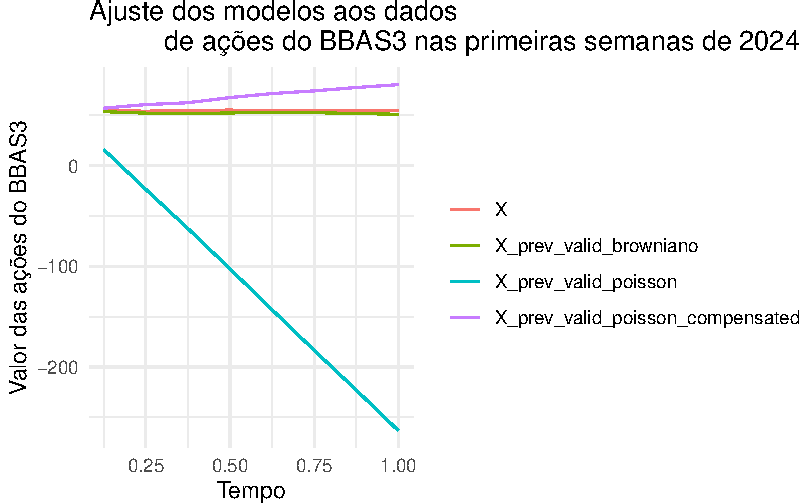
\includegraphics{questao-2_files/figure-pdf/unnamed-chunk-20-1.pdf}

}

\end{figure}

Como percebido pelo item anterior, o modelo que ajustou melhor os dados
foi o modelo estimado pelo movimento Browniano, cujo gráfico pode ser
visto a seguir:

\begin{Shaded}
\begin{Highlighting}[]
\NormalTok{dados\_valid }\SpecialCharTok{|\textgreater{}}
    \FunctionTok{filter}\NormalTok{(Variavel }\SpecialCharTok{\%in\%} \FunctionTok{c}\NormalTok{(}\StringTok{"X"}\NormalTok{, }\StringTok{"X\_prev\_valid\_browniano"}\NormalTok{)) }\SpecialCharTok{|\textgreater{}}
    \FunctionTok{ggplot}\NormalTok{() }\SpecialCharTok{+}
    \FunctionTok{geom\_line}\NormalTok{(}\FunctionTok{aes}\NormalTok{(}\AttributeTok{x =}\NormalTok{ t, }\AttributeTok{y =}\NormalTok{ Valor, }\AttributeTok{color =}\NormalTok{ Variavel)) }\SpecialCharTok{+}
    \FunctionTok{labs}\NormalTok{(}
        \AttributeTok{x =} \StringTok{"Tempo"}\NormalTok{,}
        \AttributeTok{y =} \StringTok{"Valor das ações do BBAS3"}\NormalTok{,}
        \AttributeTok{color =} \ConstantTok{NULL}\NormalTok{,}
        \AttributeTok{title =} \StringTok{"Ajuste do modelo do Movimento Browniano aos dados}
\StringTok{          de ações do BBAS3 nas primeiras semanas de 2024"}
\NormalTok{    ) }\SpecialCharTok{+}
    \FunctionTok{theme\_minimal}\NormalTok{()}
\end{Highlighting}
\end{Shaded}

\begin{figure}[H]

{\centering 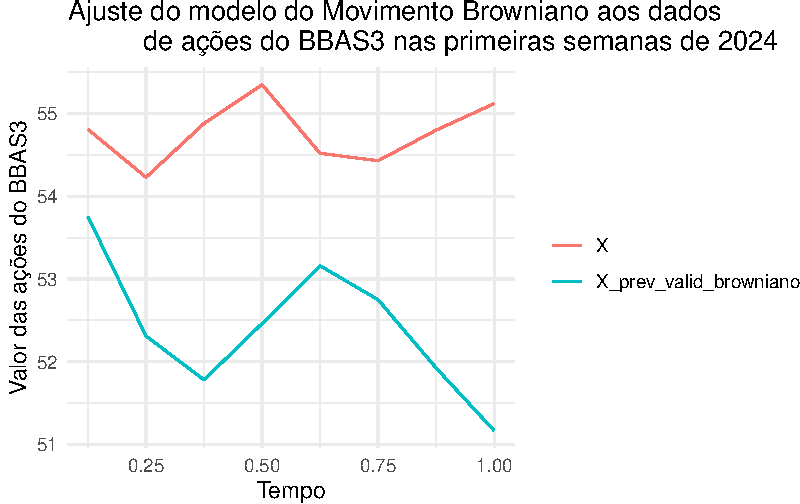
\includegraphics{questao-2_files/figure-pdf/unnamed-chunk-21-1.pdf}

}

\end{figure}

Nessa linha, o movimento Browniano parece ter melhores propriedades para
estimar e prever valores futuros das ações, marcadamente conhecidos por
alta volatilidade e comportamentos não-lineares e não-sistemáticos.



\printindex

\end{document}
